\documentclass[main.  tex]{subfiles} % Subfile-Class


% ============================================================================== %
%                            Subfile document                                    %
% ============================================================================== %

\begin{document}

\section{Konzepterstellung Antriebe}~\label{appendix:Antriebe}

Dieser Abschnitt befasst sich mit den Antrieben des Pfadfinders. Dabei werden
sowohl verschiedene Antriebskonzepte diskutiert als auch potentiell einsetzbare
Antriebe ausgewählt. Abschließend wird konzeptionell zusammengefasst, wie diese
Antriebe angesteuert werden sollen.
% ===================================================
\subsection*{Anforderungen}

\begin{description}
    \item[Beschleunigung] Eine ehrgeizige Anforderung an den Roboter ist es, ihn
          innerhalb einer Sekunde auf eine Geschwindigkeit von $2 \frac{m}{s} $
          beschleunigen zu können.
    \item[Gewicht] Das Gewicht ist, wie bei allen anderen Baugruppen, ein sehr kritischer
          Punkt bei der Entwicklung des Pfadfinders. Als \textit{Gewichtsbudget} wurde
          für die Antriebseinheit festgelegt, dass das Gewicht nicht mehr als insgesamt
          $500 g$ betragen darf.
    \item[Kosten] Das Budget für dieses Projekt ist sehr begrenzt. Der Antrieb kann ein
          wesentlicher Kostenfaktor sein, daher wurde für den Antrieb inklusive Steuerung
          und Räder ein Budget von $100 CHF$ festgelegt.
    \item[Nennspannung] Die benötigte Nennspannung des Bordnetzes hängt weitgehend von
          der benötigten Spannung der Motoren ab. Wie bereits im
          Kapitel~\ref{appendix:Bordnetz} erwähnt, würde eine Spannung von 24V ein nicht
          realisierbares Gewicht darstellen. Daher liegt die maximale Spannung für
          Motoren hier bei 12V Nennspannung.
    \item[Technik] Die Ansteuerung der Motoren ist mit geeigneten Treibern in den meisten
          Fällen relativ einfach zu realisieren. Aufgrund vorhandener Erfahrungswerte
          sollten vorzugsweise Schrittmotoren eingesetzt werden.
    \item[Schnittstelle] Die Schnittstelle zur Ansteuerung der Motoren sollte einem
          einfach zu realisierenden Standard entsprechen. Dies betrifft die Ansteuerung
          über bekannte Busprotokolle wie $I^2C$, $SPI$, $UART$ oder auch PWM- oder
          Step/Dir-Schnittstellen.

\end{description}

Die Anforderungen an die Batterie schließen aufgrund der 12V Bordnetzspannung
bereits industrietaugliche 24V Motoren aus. Diese sind zwar sehr robust, aber
in den meisten Fällen auch sehr schwer.

\newpage

\subsubsection*{Leistungsanforderungen an Motoren}
Um die Leistungsanforderungen der Motoren zu bestimmen, wurde das Beschleunigungsmoment 
berechnet, da während der Beschleunigung die grösste Last auf die Motoren wirkt. 

Abbildung~\ref{fig:Formel_Beschleunigungsmoment} zeigt die zur Berechnung verwendete 
Formel, die aus einer Maschinenbau-Formelsammlung entnommen wurde.

\begin{figure}[H]
    \centering
    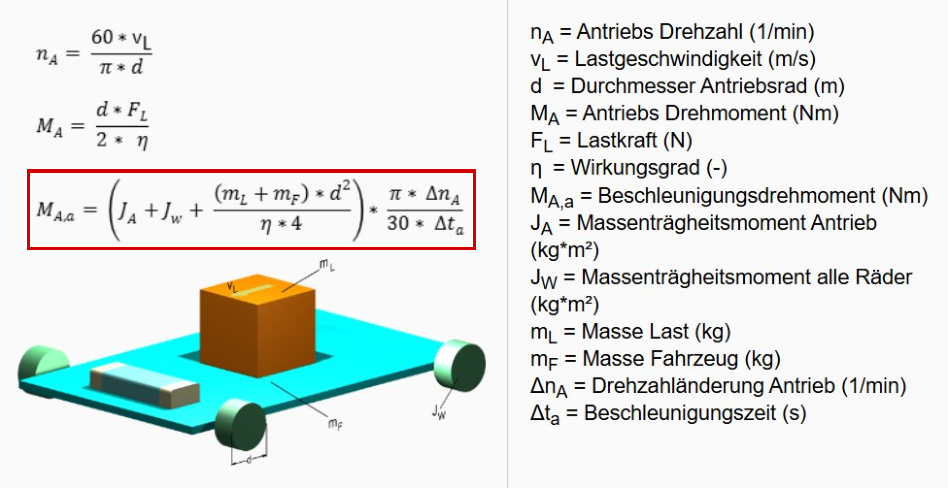
\includegraphics[width=0.7\textwidth]{./fig_Antriebe/Formel_Beschleunigungsmoment.pdf}
    \caption{Berechnungsformel aus Maschinenbau Formelsammlung}~\label{fig:Formel_Beschleunigungsmoment}
\end{figure}

Die Berechnungen wurden für alle evaluierten Motoren durchgeführt und dienten der 
Überprüfung, ob ein bestimmter Motor das erforderliche Drehmoment für die Anwendung 
liefern kann. Als Beispiel ist auf der folgenden Seite die Berechnung für den 
FIT0278-Schrittmotor von DFRobot aufgeführt.

\newpage

\textbf{Annahmen:}

\vspace{0.2cm}

Beschleunigung:
\[
a = 10 \, \si{\frac{\meter}{\second\squared}}
\]

\vspace{0.2cm}

Beschleunigungsdauer:
\[
t_{\text{Beschleunigung}} = 0.2 \, \si{\second}
\]

\vspace{0.2cm}

Wirkungsgrad des Antriebs:
\[
\eta_{\text{Antrieb}} = 0.8
\]

\vspace{0.2cm}

Max. Motorendrehzahl (keine Herstellerangabe im Datenblatt):
\[
n_{\text{Motor}} = 400 \, \si{\per\minute} 
\]

\vspace{0.5cm}

\textbf{Gegeben:}

\vspace{0.2cm}

Fahrzeuggewicht:
\[
m_{\text{Fahrzeug}} = 2 \, \si{\kilogram}
\]

\vspace{0.2cm}

Raddurchmesser:
\[
d_{\text{Rad}} = 0.08 \, \si{\meter}
\]

\vspace{0.2cm}

Masse pro Rad:
\[
m_{\text{Rad}} = 0.04 \, \si{\kilogram}
\]

\vspace{0.2cm}

Trägheitsmoment Motor:
\[
I_{\text{Motor}} = 3.5 \cdot 10^{-6} \, \si{\kilogram \cdot \meter\squared}
\]

\vspace{0.2cm}

Erdbeschleunigung:
\[
g = 9.81 \, \si{\frac{\meter}{\second\squared}}
\]

\vspace{0.2cm}

Max. Drehmoment:
\[
M_{\text{Motor, max}} = 0.343 \, \si{\newton \cdot \meter}
\]

\vspace{0.5cm}

\textbf{Berechnungen:}

\vspace{0.2cm}

Massenträgheitsmoment (zwei Räder):
\[
I_{\text{Rad}} = 2 \cdot \frac{1}{2} \cdot m_{\text{Rad}} \cdot \left( \frac{d_{\text{Rad}}}{2} \right)^2 = (6.4 \cdot 10^{-5}) \, \si{\kilogram \cdot \meter\squared}
\]

\vspace{0.2cm}

Maximale Geschwindigkeit:
\[
v_{\text{max}} = n_{\text{Motor}} \cdot d_{\text{Rad}} \cdot \pi = 1.676 \, \si{\frac{\meter}{\second}}
\]

\vspace{0.2cm}

Beschleunigungsmoment (worst case):
\[
M_{\text{max}} = \left( I_{\text{Motor}} + I_{\text{Rad}} + \frac{m_{\text{Fahrzeug}} \cdot d_{\text{Rad}}^2}{\eta_{\text{Antrieb}} \cdot 4} \right) \cdot \frac{\pi \cdot n_{\text{Motor}}}{t_{\text{Beschleunigung}}} = 0.426 \, \si{\newton \cdot \meter}
\]

\vspace{0.2cm}

Drehmoment pro Motor:
\[
M_{\text{Motor}} = \frac{M_{\text{max}}}{2} = 0.213 \, \si{\newton\cdot \meter}
\]

% ===================================================
\newpage

\subsection*{Konzeption}

Ausgehend von den Leistungsanforderungen an die Motoren kann am Markt
recherchiert werden, welche Motoren potenziell verfügbar sind. Diese können
wiederum nach den Kriterien Kosten, Gewicht, Leistung und Entwicklungsaufwand
miteinander verglichen werden.

\subsubsection*{Konzept 1 - Bipolarer Schrittmotor} % =========

Die Wahl fällt auf einen bipolaren Schrittmotor, da dieser bei gleichem Gewicht
eine bessere Ausnutzung der Spulen und damit eine höhere Leistung bei gleichem
Gewicht im Vergleich zu einem unipolaren Schrittmotor ermöglicht. Ein Vergleich
verschiedener Schrittmotoren hat gezeigt, dass Schrittmotoren, die in einem
Nennstrombereich von $1. 2A$ bis $2A$ liegen, in einem Bereich liegen, der die
Leistungsanforderungen bereits ohne Zwischengetriebe erfüllen kann. Typische,
kostengünstige Vertreter dieser Reihe sind die
inTabelle~\ref{tab:Schrittmotoren_different} aufgeführten.

\begin{table}[h]
    \centering
    \begin{tabular}{|p{2cm}|p{3cm}|p{2cm}|p{1cm}|p{1cm}|p{1cm}|p{1.5cm}|}
        \hline
        Hersteller           & Herst.Nr       & Distributor  & $I_{nenn} $ [A] & $U_{nenn}$ [V] & Preis [CHF] & Gewicht [kg] \\ \hline
        Olimex LTD           & SM-42HB34F08AB & DigiKey.ch   & 1.  33          & 12             & 9.36        & 0.400        \\ \hline
        DFRobot              & FIT0278        & DigiKey.ch   & 1.  7           & 3.4            & 12          & 0.269        \\ \hline
        SparkFun Electronics & ROB-10846      & DigiKey.ch   & 1.  7           & 3              & 16.77       & 0.356        \\ \hline
    \end{tabular}
    \caption{Verschiedene Schrittmotoren}
    \label{tab:Schrittmotoren_different}
\end{table}

Dieser Vergleich zeigt, dass sich eigentlich nur der Motor \textit{FIT0278}
von\textit{DFRobot} in einem akzeptablen Verhältnis von Gewicht und Leistung
befindet. Alle aufgeführten Motoren sind preisgünstig. Die Motoren müssen über
gekaufte Treiber angesteuert werden. Die Eigenentwicklung eines Motortreibers
ist zwar mit wenig Aufwand zu realisieren,fertige Treiberendstufen sind jedoch
sehr preisgünstig und einfach anzusteuern. Bei der Ansteuerung des
Schrittmotorentreibers \textit{TMC5240} von \textit{ADI-Trinamic} kann ein
Teammitglied auf Erfahrungen aus seinem beruflichen Umfeld zurückgreifen. Diese
Treiber stehen auch für dieses Projekt in zweifacher Ausführung zur Verfügung.
Der Vergleich dieses Treibers mit einem einfach anzusteuernden Treiber zeigt
die Tabelle~\ref{tab:Schrittmotorentreiber_different}.

\begin{table}[h]
    \centering
    \begin{tabular}{|p{2cm}|p{3cm}|p{2cm}|p{1cm}|p{1cm}|p{1cm}|p{1.5cm}|}
        \hline
        Hersteller & Herst.Nr   & Distributor   & $I_{nenn} $ [A] & $U_{nenn}$ [V] & Preis [CHF] & Gewicht [kg] \\ \hline
        ADI        & TMC5240-EVAL & Komax AG      & 2               & 36             & 63          & 0.036      \\ \hline
        ACT Motor  & ACT DM430    & reichelt.ch & 3               & 32             & 17.42     & 0.180      \\ \hline
    \end{tabular}
    \caption{Verschiedene Schrittmotorentreiber}
    \label{tab:Schrittmotorentreiber_different}
\end{table}

\subsubsection*{Konzept 2 - Radnabenmotor} % =========

Auf dem Markt sind fertige Radnaben erhältlich, die zum Teil bereits sowohl
Endstufen als auch eine Steuerung enthalten:

\begin{table}[h]
    \centering
    \begin{tabular}{|p{2cm}|p{3cm}|p{2cm}|p{1cm}|p{1cm}|p{1cm}|p{1.5cm}|}
        \hline
        Hersteller & Herst.Nr & Distributor  & $I_{nenn} $ [A] & $U_{nenn}$ [V] & Preis [CHF] & Gewicht [kg] \\ \hline
        DFRobot    & FIT1001& DigiKey.ch & 0.5& 14.4& 25.71& 0.216\\ \hline
    \end{tabular}
    \caption{Radnabenmotor DFRobot}
\end{table}

Der gezeigte Motor ist einfach über den UART-Bus anzusteuern, kostengünstig,
leicht und hat einen integrierten Encoder. Ein großer Nachteil ist jedoch, dass
mit diesem Motor das ehrgeizige Ziel einer Beschleunigung von $2 \frac{m}{s^2}$
voraussichtlich nicht erreicht werden kann.

\subsection*{Konzept 3 - BLDC-Motor} % =========

BLDC-Motoren haben den großen Vorteil, dass sie eine hohe Leistung bei geringem
Gewicht erreichen können. Allerdings ist ihr Drehmoment eher gering, weshalb
ein Zwischengetriebe notwendig ist. Dieses Zwischengetriebe erhöht das Gewicht
des Antriebs zusätzlich. Außerdem sind BLDC-Motoren oft teurer. In der
folgenden Tabelle sind verschiedene Motoren aufgelistet, die in Frage kommen.
% YANIK FRAGEN DER DFROBOT KÖNNTE NOCH SPANNEND SEIN !!!!!!!!!!!!!!!!!!!!!!!!!!!!!!!!!!!!!!!!

\begin{table}[h]
    \centering
    \begin{tabular}{|p{2cm}|p{3cm}|p{2cm}|p{1cm}|p{1cm}|p{1cm}|p{1.5cm}|}
        \hline
        Hersteller      & Herst.Nr    & Distributor  & $I_{nenn} $ [A] & $U_{nenn}$ [V] & Preis [CHF] & Gewicht [kg] \\ \hline
        DFRobot         & FIT0441       & DigiKey.ch & 0.7           & 12             & 17.11     & 0.070      \\ \hline
        Lin Engineering & BL17E19-01-RO & DigiKey.ch &                 & 24             & 79.18     & 0.320      \\ \hline
    \end{tabular}
    \caption{Radnabenmotor DFRobot}
\end{table}

Der Motor von DFRobot wird mit seiner Geschwindigkeit von maximal $159
    \frac{1}{min}$ zwar nicht die gewünschte Drehzahl erreichen, aber das geringe
Gewicht bei entsprechender Leistung sowie der bereits integrierte Treiber
machen diesen Antrieb dennoch wert, im Detail evaluiert zu werden. Generell hat
die Komponentenrecherche ergeben, dass BLDC-Motoren eine höhere Nennspannung
benötigen, als mit dem dimensionierten Akkupack zur Verfügung gestellt werden
kann. Als Stromquelle dienen natürlich Motortreiber, jedoch werden Motoren im
entsprechend benötigten Leistungsbereich schnell zu teuer und zu schwer.
Generell können BLDC-Motoren, ähnlich wie Schrittmotoren, über einen selbst
entwickelten Treiber angesteuert werden, aber auch fertige Motorsteuerungen
sind unschlagbar günstig und über eine PWM-Schnittstelle sehr einfach
anzusteuern. Stellvertretend für diese Produktgruppe sei der folgende Motor
genannt.

\begin{table}[h]
    \centering
    \begin{tabular}{|p{2cm}|p{3cm}|p{2cm}|p{1cm}|p{1cm}|p{1cm}|p{1.5cm}|}
        \hline
        Hersteller & Herst.Nr   & Distributor & $I_{nenn} $ [A] & $U_{nenn}$ [V] & Preis [CHF] & Gewicht [kg] \\ \hline
        ACT Motor  & BLDC-8015A-5 & reichelt.ch & 15              & 50             & 39.1      & 0.432      \\ \hline
    \end{tabular}
    \caption{BLDC-Treiber}
\end{table}

\subsubsection*{Fazit und Entscheid aus der Konzeptionsphase}  % =========

In der Gruppe wurde beschlossen, den in Abbildung~\ref{fig:DFROBOT_FIT0278}
dargestellten Schrittmotor von DFRobot in Kombination mit den in
Abbildung~\ref{fig:TMC5240_EVAL} dargestellten Schrittmotorentreibern von
Trinamic genauer zu analysieren und zu verfolgen. Als\textit{Plan-B}, auch für
den Fall, dass das gewünschte Gewicht nicht eingehalten werden kann, soll der
Radnabenmotor, ebenfalls von DFRobot, evaluiert werden. Damit können zwar nicht
unbedingt die gewünschten Geschwindigkeits- und Beschleunigungswerte erreicht
werden, aber die Ansteuerung ist sehr einfach, die Treiber sind bereits
integriert und zudem sind sie leicht.

\begin{figure}[h!]
    \centering
    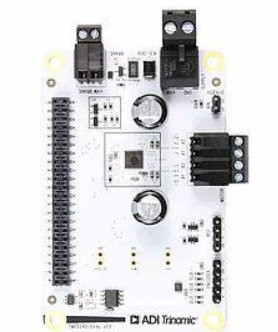
\includegraphics[width=0.25\textwidth]{./fig_Antriebe/TMC_5240_EVAL.png}
    \caption{TMC 5240 Evaluation-Board}~\label{fig:TMC5240_EVAL}
\end{figure}

\begin{figure}[h!]
    \centering
    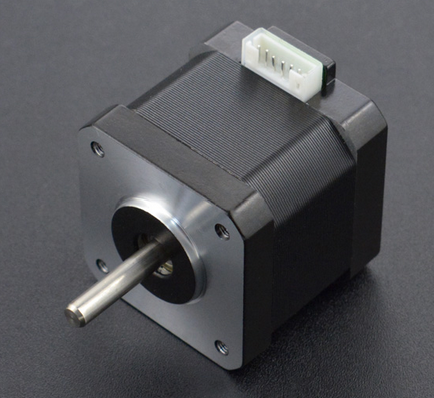
\includegraphics[width=0.25\textwidth]{./fig_Antriebe/DFRobot_Stepper_FIT0278.png}
    \caption{DFROBOT FIT0278 Schrittmotor}~\label{fig:DFROBOT_FIT0278}
\end{figure}

Dieser Motor soll durch einen echtzeitfähigen Mikroprozessor geregelt werden,
dem auch die Sensordaten des Liniensensors zur Verfügung stehen. Der Antrieb
soll auf das Feedback dieses Sensors geregelt werden. Dies ist in
Abbildung~\ref{fig:RTC_Trinamic_Konzept} nochmals verdeutlicht.
\begin{figure}[h!]
    \centering
    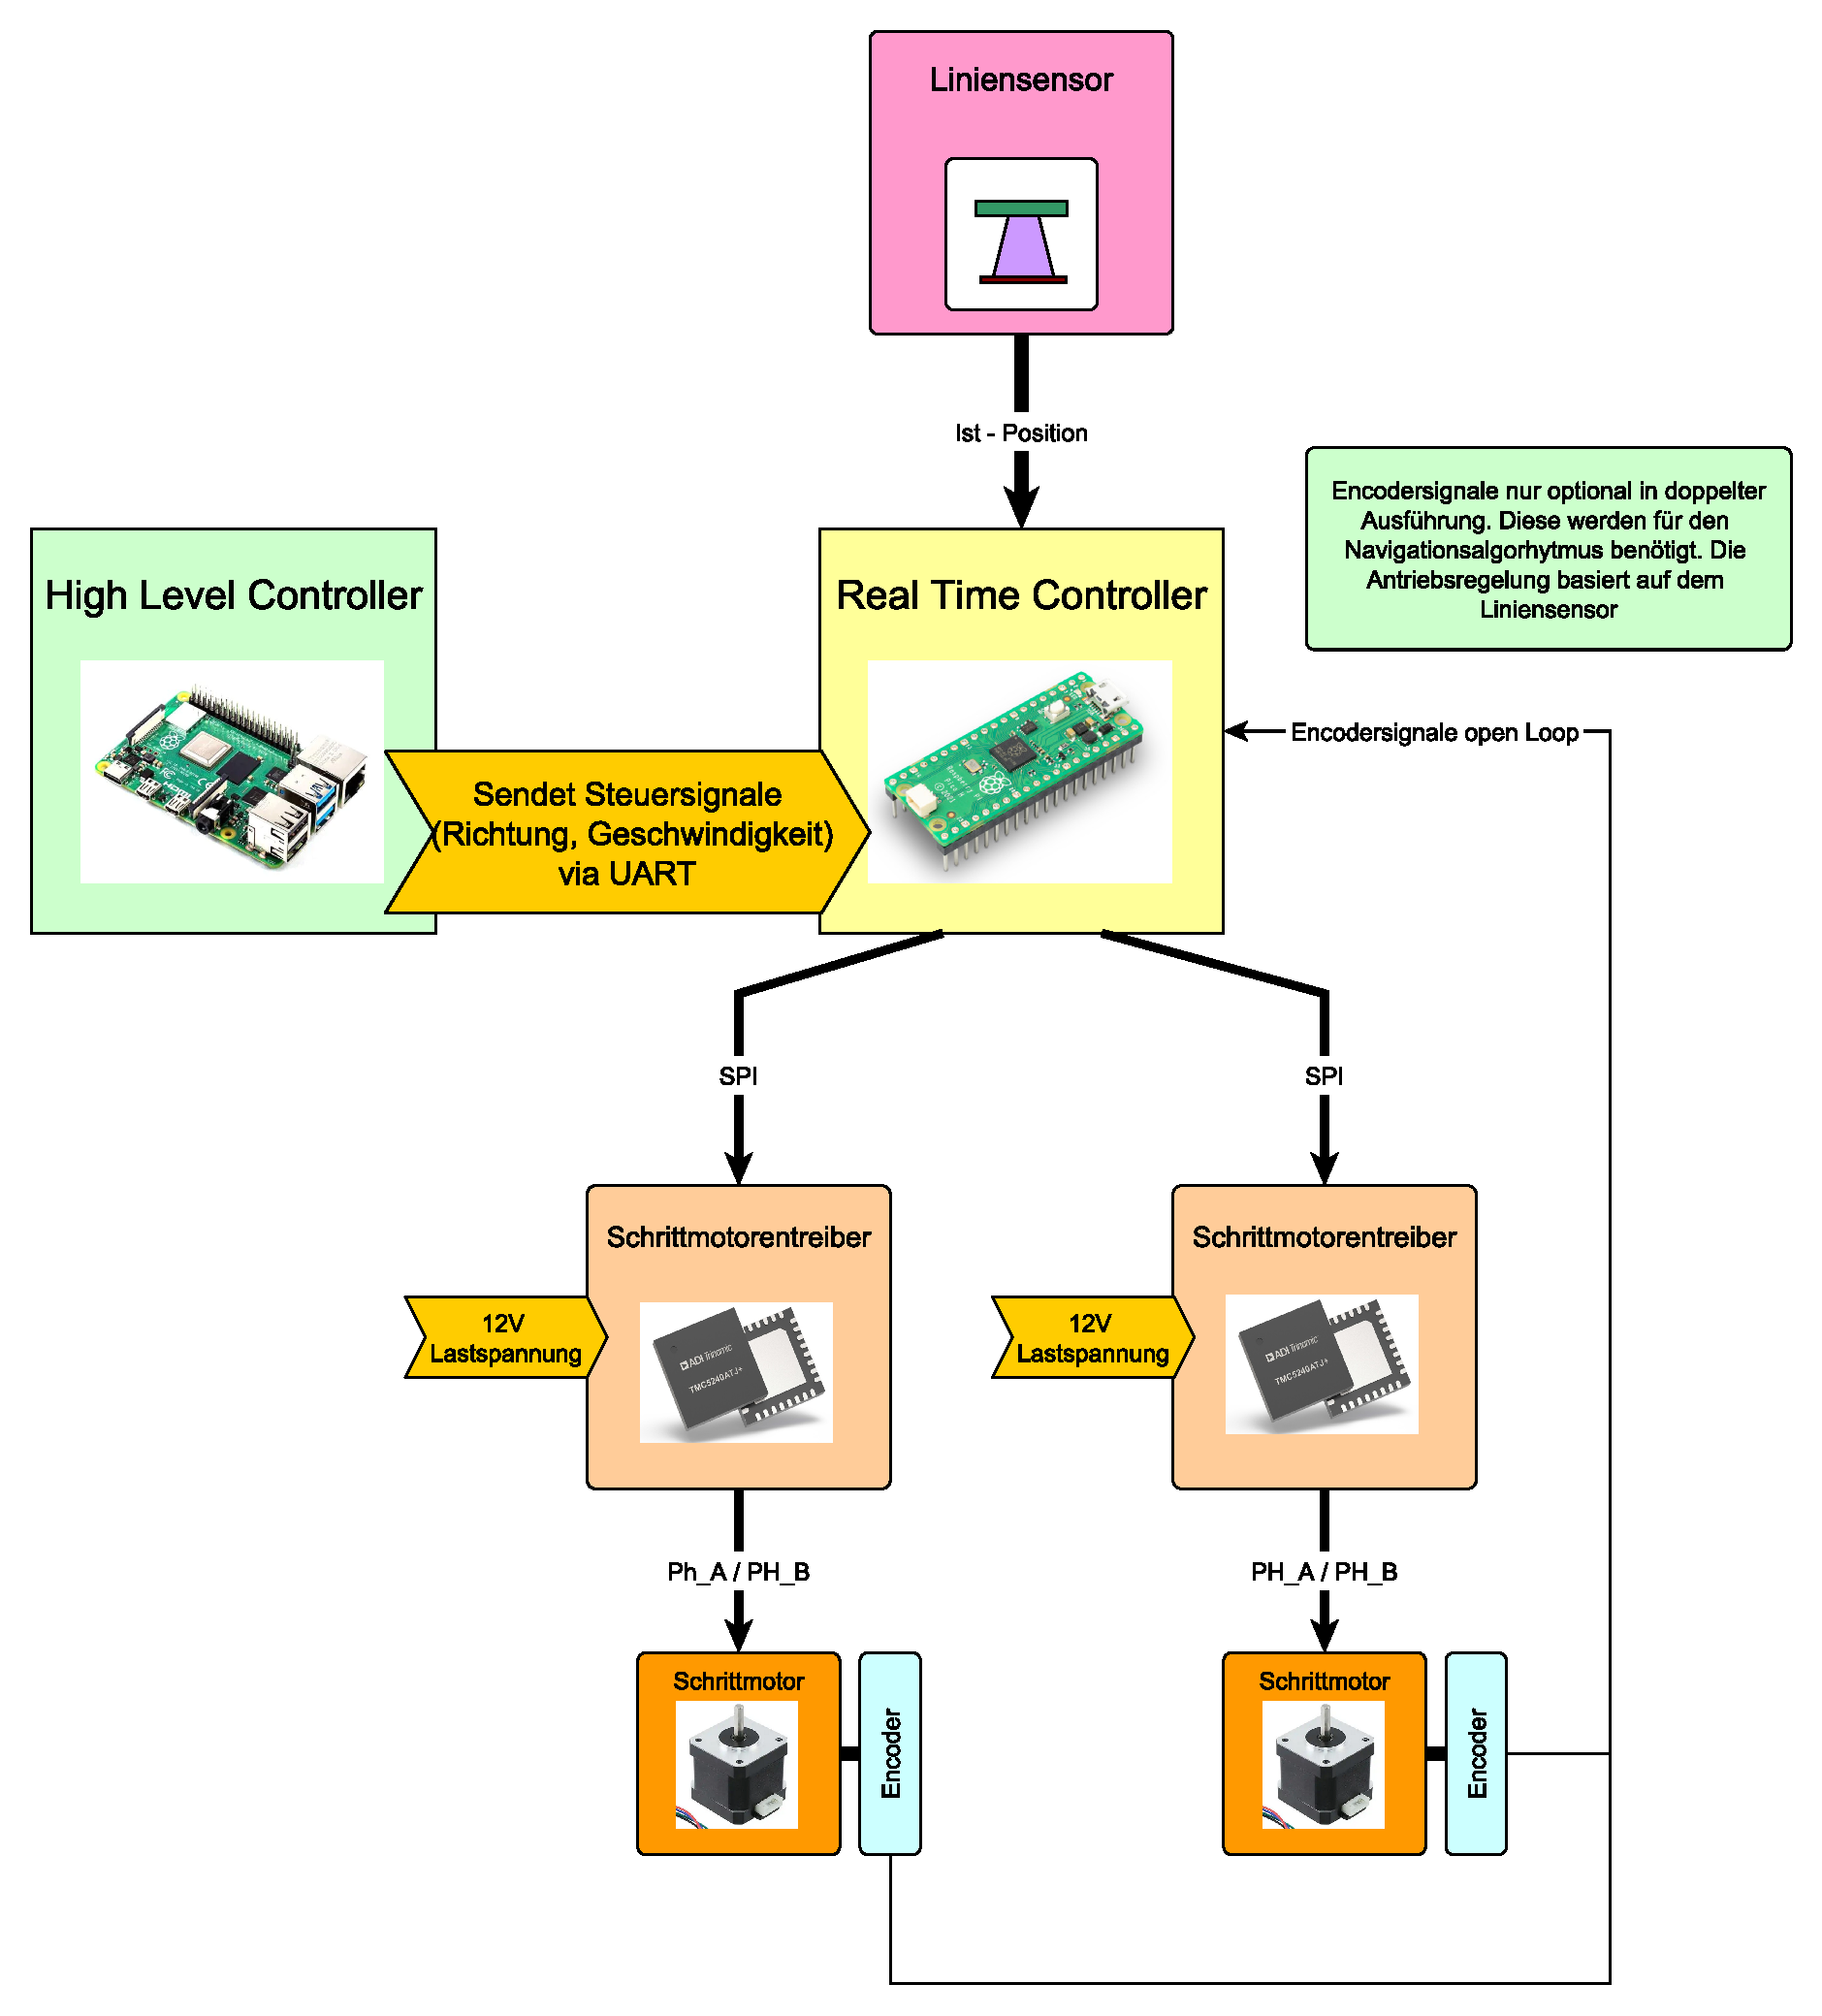
\includegraphics[width=0.75\textwidth]{./fig_Antriebe/Konzept_RTC_Trinamic.pdf}
    \caption{Konzept für die Ansteuerung der Schrittmotoren}~\label{fig:RTC_Trinamic_Konzept}
\end{figure}

Zusätzlich ist mindestens ein Encoder vorgesehen, der mit einer einfachen
Lochscheibe und einer Gabellichtschranke realisiert ist. Dieser hat jedoch
keine Anwendung in der Fahrzeugregelung. Er dient lediglich zur Erfassung der
zurückgelegten Wegstrecke. Die ausgewählten Antriebe könnten direkt über den
High-Level-Controller angesteuert werden. Die Antriebsregelung wurde jedoch
bewusst auf einen Mikroprozessor verlagert, um dem Ansatz der Gewaltentrennung
gerecht zu werden. So gibt es einen echtzeitfähigen Prozessor, der sich
ausschließlich um die Lageregelung kümmert, während der High-Level-Controller
lediglich die Richtungsentscheidungen trifft.

\subsection*{Motion Controller} % =========

Für die Integration der Schrittmotortreiber in das Gesamtsystem wird eine
eigene Leiterplatte entwickelt. Der komplette Schaltplan befindet sich im
Anhang. Im Folgenden wird auf einige Baugruppen näher eingegangen.
\subsubsection*{Anforderungen}

\begin{description}
    \item[Spannungsversorgung] Die Leiterplatte muss mit 12V versorgt werden können.
    \item[Digitale Ein- und Ausgänge] Die Leiterplatte muss über digitale Ein- und
          Ausgänge mit Spannungsversorgung verfügen. Es müssen sowohl industrietaugliche
          12V als auch 3V3 Sensoren betrieben werden können. Ausgänge sollen sowohl
          Lasten Schalten, aber auch logische Signale übertragen können.
    \item[Analoge Eingänge] Der PCB muss in der Lage sein, mit 8 analogen Eingängen den
          Liniensensor auswerten zu können.
    \item[Kommunikationsschnittstellen] Der Motion Controller muss 2 Punkt zu Punkt UART
          Kommunikation über eine RS422 Schnittstelle aufbauen können.
    \item[Motorentreiber Schnittstellen] Die Motorentreiber sollen möglichst einfach
          angeschlossen werden können, es ist erwünscht, dass der MotionController
          einfach aufgesteckt werden kann.
    \item[Gyroskop] Das PCB muss über eine Möglichkeit der Winkelerfassung verfügen.
    \item[HC-SR04 Schnittstelle] Das PCB muss einen Ultraschallsensor auswerten können.
    \item[Debugfunktionen] Einzelne Signale können zusätzlich auf LEDs gelegt werden, um
          sie für Debugzwecke sichtbar zu machen.
    \item[Baugröße] Die Platine darf maximal 100mm x 100mm groß sein, da dadurch massiv
          Kosten gespart werden können.
\end{description}

\subsubsection*{Schaltungsbeschreibung}

\paragraph{Spannungsversorgung}

Die Leiterplatte wird mit einer Spannung von 12V versorgt. Diese 12V werden
zunächst mit einem DC-DC-Wandler auf 5,5V heruntergeregelt, bevor sie über 2
LDOs zunächst auf 5V und dann nochmals auf 3,3V heruntergeregelt werden.
Abbildung~\ref{fig:Schema_Spannungsversorgung} zeigt genau diese Schaltung.

\begin{figure}[h!]
    \centering
    \includegraphics[page=2,width=\textwidth]{../Anhang_pdfs/MotionController.pdf}
    \caption{Auszug Schema Spannungsversorgung}~\label{fig:Schema_Spannungsversorgung}
\end{figure}

\paragraph{Verbindungen an TMC5240}
Die Abbildung~\ref{fig:Schema_TMC5240} zeigt, wie die Motortreiber über 2
44-polige Steckerleisten einfach auf den Motion Controller aufgesteckt werden
können. 2 LEDs zeigen die aktuell gewählte Strombegrenzung an.

\begin{figure}[h!]
    \centering
    \includegraphics[page=3,width=\textwidth]{../Anhang_pdfs/MotionController.pdf}
    \caption{Auszug Schema TMC5240 - Anbindung}~\label{fig:Schema_TMC5240}
\end{figure}

\paragraph{Kommunikationsschnittstellen}
Abbildung~\ref{fig:Schema_Kommunikation} zeigt den Anschluss der beiden
Kommunikationskanäle \textit{UART\_0} und \textit{UART\_1} an zwei separate
RS422-Schnittstellen. Prinzipiell sind UART-Kanäle Push-Pull-Stufen -
allerdings sind diese Zustände beim Systemstart noch nicht zwingend definiert.
Um Bit-Banging auf der Kommunikationsleitung zu vermeiden, sind diese Signale
dennoch mit Pullup-Widerständen versehen.

\begin{figure}[h!]
    \centering
    \includegraphics[page=4,width=\textwidth]{../Anhang_pdfs/MotionController.pdf}
    \caption{Auszug Schema Kommunikationsschnittstellen}~\label{fig:Schema_Kommunikation}
\end{figure}

\paragraph{Digital Eingänge}
Abbildung~\ref{fig:Schema_DInput} zeigt einen digitalen Eingang des Motion
Controllers. 2 der 4 Eingänge können sowohl mit 12V als auch mit 3V3 versorgt
und geschaltet werden. Um den Eingang auf 3V3 umzukonfigurieren müssen
lediglich die beiden Jumper am Eingang gesetzt werden, die anderen beiden
digitalen Eingänge sind fest auf 12V konfiguriert. Das eingehende Signal wird
über ein RC-Glied und einen Schmitt-Trigger entprellt. Eine LED zeigt an, dass
der Eingang geschaltet ist.

\begin{figure}[h!]
    \centering
    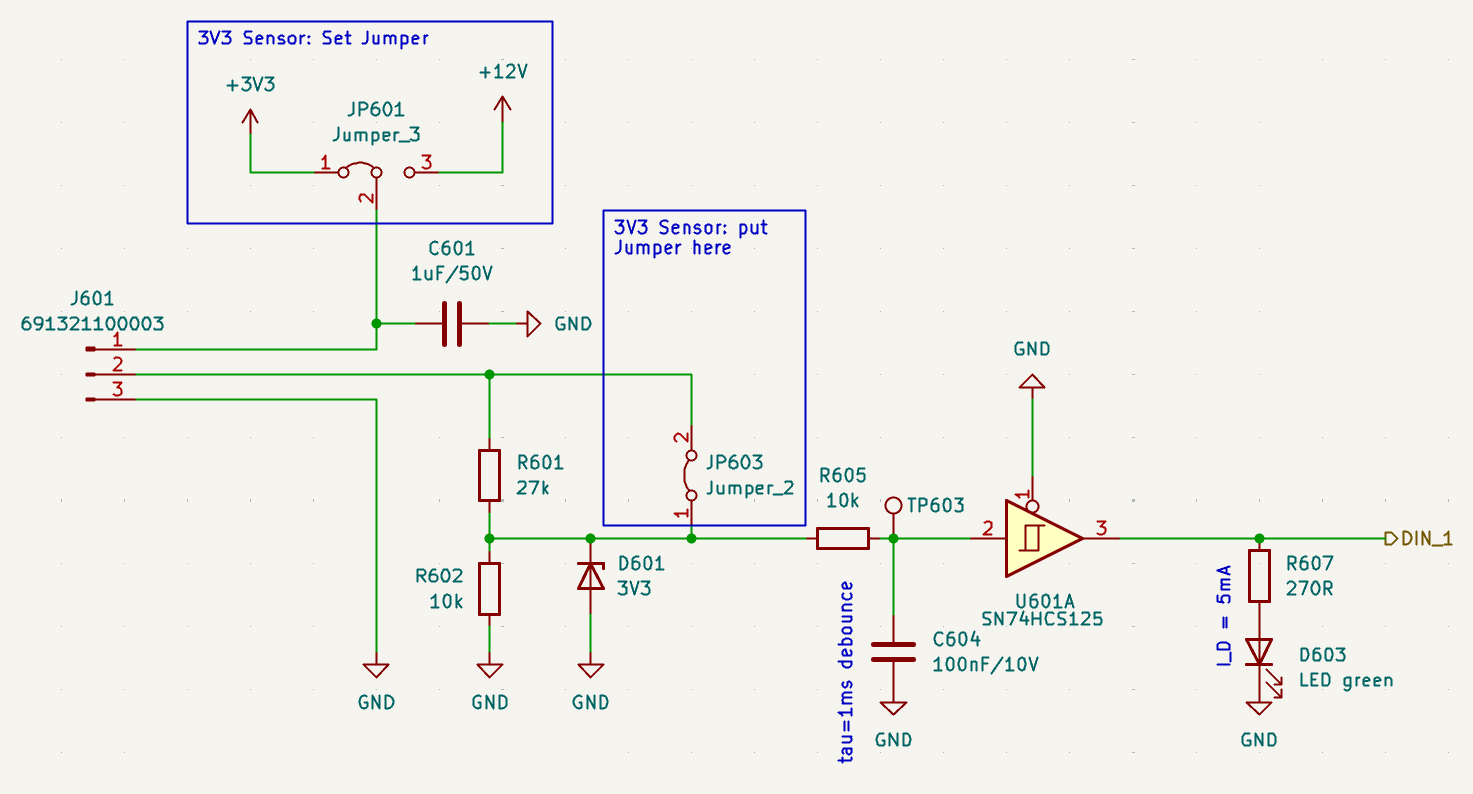
\includegraphics[width=0.5\textwidth]{./fig_Antriebe/Schema_DIN_Umschaltbar.png}
    \caption{Auszug Schema Digitaler Eingang}~\label{fig:Schema_DInput}
\end{figure}

\paragraph{Analoge Eingänge}
Abbildung~\ref{fig:Schema_AIn} zeigt den Anschluss der Analogsignale an den
Raspberry Pico. Es wird ein $I^2C$-fähiger ADC mit 8 Eingängen verwendet. Die
eingehenden Signale werden über einen RC-Tiefpass gefiltert. Weiterhin kann die
Versorgungsspannung der Liniensensor-Sender ein- und ausgeschaltet werden.
Dadurch ist es möglich, den Sensor bei Bedarf nur dann einzuschalten, wenn
gerade gemessen wird. UV-Strahlung ist für das menschliche Auge schädlich und
kann so zum Personenschutz beitragen.

\begin{figure}[h!]
    \centering
    \includegraphics[page=7,width=\textwidth]{../Anhang_pdfs/MotionController.pdf}
    \caption{Auszug Schema Analogeingänge}~\label{fig:Schema_AIn}
\end{figure}

\paragraph{Digitale Ausgänge}
Abbildung~\ref{fig:Schema_DOut} zeigt die 4 digitalen Ausgänge des Motion
Controllers. Über die beiden Ausgänge DOUT\_1 und DOUT\_2 können größere Ströme
mit jeweils 5V5 bzw. 12V geschaltet werden. Der gezeigte High-Side Switch
erlaubt Ströme bis zu 3A. Die beiden rechten Ausgänge sind für logische
Ausgangspegel vorgesehen. Über sie kann z.B. auch ein PWM-Signal ausgegeben
werden. Die Pull-Down-Widerstände ermöglichen einen schnellen Übergang nach
GND, wenn logische Rechtecksignale schnell geschaltet werden müssen.

\begin{figure}[h!]
    \centering
    \includegraphics[page=8,width=\textwidth]{../Anhang_pdfs/MotionController.pdf}
    \caption{Auszug Schema Digitale Ausgänge}~\label{fig:Schema_DOut}
\end{figure}

\paragraph{I2C Schnittstellen}
In der Abbildung~\ref{fig:Schema_I2C} sind 3 $I^2C$-Schnittstellen dargestellt.
Der Motion Controller verfügt über 2 I2C-Schnittstellen, die auf einem
3V3-Pegel arbeiten und eine, die auf einem 5V-Pegel arbeitet. An diese
Schnittstellen können Sensoren wie Lidar oder auch LCD Displays angeschlossen
werden.

\begin{figure}[h!]
    \centering
    \includegraphics[page=9,width=\textwidth]{../Anhang_pdfs/MotionController.pdf}
    \caption{Auszug Schema I2C Verbindungen}~\label{fig:Schema_I2C}
\end{figure}

\paragraph{Gyroskop und Ultraschallsensor}
Diese Schaltung ist in Abbildung\ref{fig:Schema_sonstige_Sensoren} dargestellt.
Das Gyroskop ist sehr rudimentär angeschlossen und verzichtet auf viele
Funktionen, da es diese schlichtweg nicht benötigt. Falls wider Erwarten doch
mit einem Interrupt gearbeitet wird, ist zumindest einer angeschlossen. Der
Ultraschallsensor HC-SR04 arbeitet auf einem 5V-Pegel und wird über einen
MOSFET angesteuert. Damit das Echo-Signal den Eingang nicht beschädigt, wird
der Spannungspegel über einen Spannungsteiler auf 3,3V reduziert.

\begin{figure}[h!]
    \centering
    \includegraphics[page=10,width=\textwidth]{../Anhang_pdfs/MotionController.pdf}
    \caption{Auszug Schema Gyroskop und HCSR-04}~\label{fig:Schema_sonstige_Sensoren}
\end{figure}

\end{document}
